%!TEX root = spadini_davide.tex

\chapter{Wormhole Peer Sampling Service}
\label{cha:wormhole}
\ac{WPSS}~\cite{wormhole} is an algorithm written by Roberto Roverso, Jim Dowling and Mark Jelasity, published in 2013. It has been presented in the $13^{th}$ IEEE International Conference on Peer-to-Peer Computing. In the original paper it has been proved, compared to the state of the art at that time, that it has the same levels of samples' freshness  of the other peer sampling services, while the connection establishment rate is decreased by one order of magnitude. Another important feature is that it is a NAT-aware protocol, meaning that it handles situations in which some peers are behind NATs or firewall.

In the next sections we are going to see the reasons why these previous aspects might benefit our purpose, and how the algorithm really works.

\section{Peer Sampling Service}
\label{sec:pss}
A peer sampling service (PSS) is a service that runs on all the nodes in a distributed system and provides them with a uniform random sample of live nodes from the system, where the sample size is typically much smaller than the system size. 

The reason beyond this service is that, while in the past we had that the network was relatively small and all the nodes had the full view of it (it was almost a static network), now this is not the case anymore: in fact a general distributed system like a peer-to-peer system may contain a lot of peers which can join, leave or crash at any time. In this system, having a complete view of the network could be useless or even impossible, so the peer sampling service provides a list of ``fresh'' nodes which reflects the peers known by the node inside the network.

A PSS can be implemented as a centralized service~\cite{spotify}, using gossip protocols~\cite{gossip_protocol} or random walks~\cite{rw}. Gossip-based PSSes have been the most widely adopted solution, as centralized PSSes are expensive to run reliably, and random walks are only suitable for stable networks~\cite{rw}. However, in the Internet, where a high percentage of nodes are behind NATs, these traditional gossip-based PSSes become biased. Nodes cannot establish direct connections to nodes behind NATs (\emph{private nodes}), and private nodes become under-represented in partial views, while nodes that do support direct connectivity, \emph{public nodes}, become over-represented in partial views~\cite{gozar}. 

So to overcome the problem, a new class of NAT-aware gossip-based PSSes have appeared to be able to generate uniformly random node samples even for systems with a high percentage of private nodes, that is, nodes that reside behind a NAT and/or firewall.

State of the art NAT-aware gossip protocols, such as Gozar~\cite{gozar} and Croupier~\cite{croupier}, require peers to frequently establish network connections and exchange messages with public nodes, nodes that support direct connectivity, in order to build a view of the overlay network. However, in commercial P2P applications such as Spotify~\cite{spotify}, P2P-Skype~\cite{skype} and as we saw in Sect.~\ref{sec:webrtc_api} Google’s WebRTC, establishing a connection is a relatively complex and costly procedure. First of all because privacy is a concern, all new connections require peers to authenticate the other party with a secure server and to setup an encrypted channel. Another reason is that establishing a new connection may involve coordination by a helper service, for instance, to work around connectivity limitations that are not captured by NAT detection algorithms, e.g. using STUN Servers (Sect.~\ref{sec:webrtc_ice}). 

In~\cite{wormhole} they show that \ac{WPSS} can provide the same level of freshness of samples as the state of the art in NAT-aware PSSes~\cite{croupier} but with a connection establishment rate that is one order of magnitude lower. This, without sacrificing the desirable properties of a PSS for the Internet, such as robustness to churn, NAT-friendliness and local randomness of samples.

\section{WPSS: the algorithm}
\label{sec:wpss_algorithm}
The main idea behind \ac{WPSS} is that the service is separated into two layers. The bottom layer consists of a stable base overlay network that should be NAT-friendly, with private nodes connecting to public nodes, while public nodes connect to one another. The number of links in the base overlay is fixed at bootstrap-time and it is maintained during all the duration of the algorithm using the tracker (see Sect.~\ref{cha:tracker}) to replace the broken links with new ones.

On top of that there is the Wormhole overlay: every node periodically connects to a public node selected randomly from the base overlay (but not necessarily a neighbour). These links to random public nodes are called wormholes: each node systematically places samples of itself on nodes in the neighbourhood of their wormhole. 

Fig.~\ref{fig:overlay} shows this mechanism: in the bottom layer, the stable base overlay, there are private nodes connected to public nodes, and public nodes connected to one another; the upper layer, the wormhole overlay, shows a node with its wormhole placing samples of itself in the neighbourhood.

\begin{figure}[ht]
  \centering
  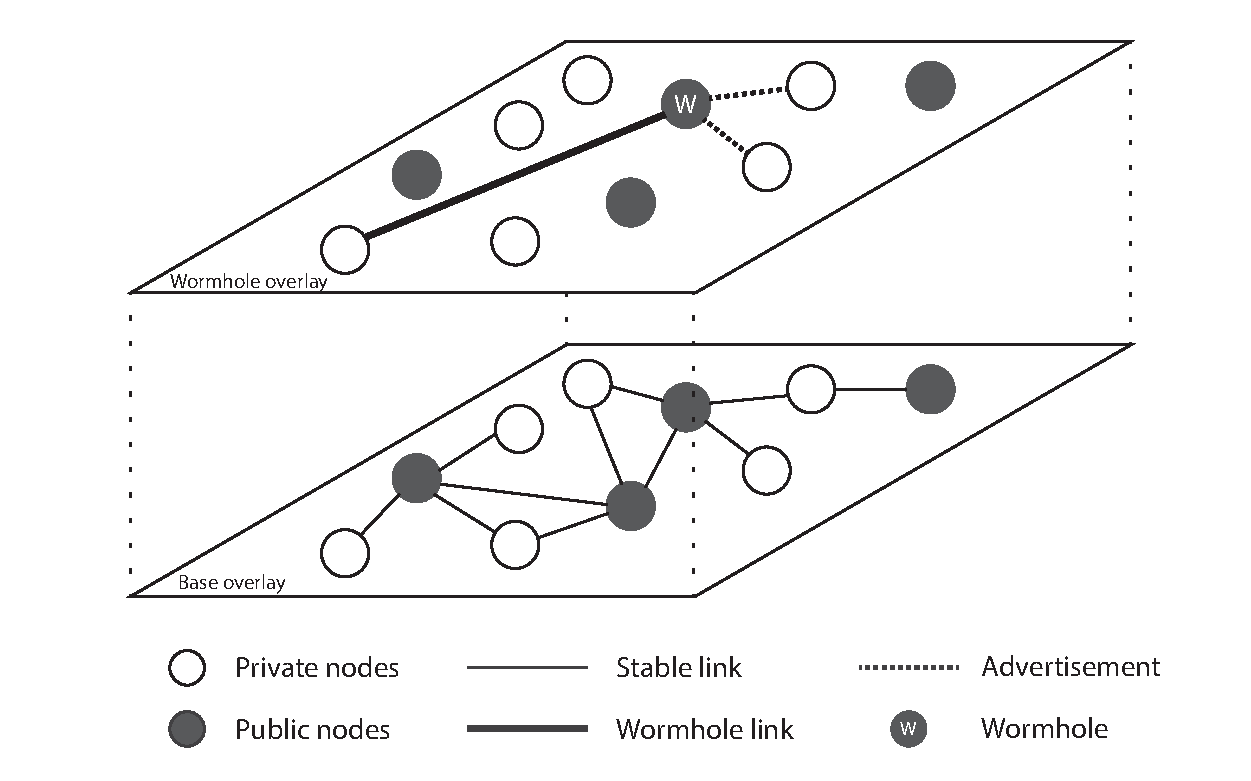
\includegraphics[keepaspectratio=true, width=\textwidth]{images/overlay.pdf}\caption{The difference between the two overlays}
  \label{fig:overlay}
\end{figure}

In other words, when the nodes start they ask the tracker the reference of $N$ random public nodes: that will be their base overlay. Then, they periodically disseminate (push) advertisements of themselves over a small number of hops traversing the wormhole link and they place it at the node where this (typically short) walk terminates.

As explained before, a wormhole link points to a public node in the system that is selected independently at random. In \ac{WPSS} every node discovers such a random public node to act as its wormhole, and every node only has one wormhole active at any given point in time. A new network connection will be created only when a wormhole is traversed for the first time by an advertisement. The wormhole is then reused for a few subsequent advertisements from the same initiator node, in which case no new network connection needs to be established. This makes it possible to decrease the number of new links established.

The very first time an advertisement reaches the wormhole, it can be placed at the public node as a new sample. However, if the public node already has a sample from the initiator node, then the advertisement will start a random walk over the base overlay until it either reaches a node that does not already have a sample from the initiator node or it reaches a given time-to-live (TTL)~\cite{wormhole}.

So, the first time a node will send the advertisement to its wormhole will create a link to it and it will place a sample first at that public node unless it already has an advertisement from the initiator. However, the reuse of the wormhole causes advertisements to continue, allowing them to also finish at private nodes, as private nodes are connected to public nodes over the base overlay. 

When a wormhole is re-used by an advertisement, the expected number of hops the advertisement will have to take increases, as it needs to reach a node that does not already have a sample from the initiator node. To counteract this, the \ac{WPSS} defines a ``wormhole renewal period'' as a parameter for creating new wormholes, enabling users to control how frequently new network connections will be created. We will see in Sect.~\ref{cha:evaluation} that tuning this parameter is very important. 


\begin{algorithm}[H]
  \SetKwProg{Upon}{upon}{ do}{end}
  \SetKwProg{Every}{every}{ do}{end}

  \Upon{wormholeFailure}{
  	$wormhole \leftarrow tracker.getNewWormhole()$\;
    $connect(wormhole)$
  }

  \Upon{baseOverlayFailure}{
  	$peer \leftarrow tracker.getNewPeer()$\;
  	$connect(peer)$
  }

  \Every{$\Delta_{wh}$ = wormholeTimeout}{
    $disconnect(wormhole)$\;
  	$wormhole \leftarrow tracker.getNewWormhole()$\;
    $connect(wormhole)$\;
  }

  \Every{$\Delta$ = adTimeout}{
  	$ad \leftarrow createAd()$\;
  	$ad.hops \leftarrow 1$\;
  	$sendAdToWormhole(wormhole, ad)$\;
  }

  \Upon{receivedAd(ad)}{
  	\If{ad.hop = getTTL() $\mid\mid$ acceptAd(ad)}{
  		view.addAd(ad)
  	}\Else{
  		$neighbour \leftarrow getMetropolisHastingsNeighbour(baseOverlay)$\;
  		$ad.hop \leftarrow ad.hop + 1$\;
  		$sendAd(j, ad)$\;
  	}
  }

 \caption{Wormhole peer sampling}
\end{algorithm}

\textbf{Algorithm 1} shows the pseudo-code of the \ac{WPSS}. The algorithm runs on all the peers (private and public) in the same way and contains three event-handlers and two timers. 

The event-handlers are: \wormholeFailure, \baseOverlayFailure and \receivedAd. The first two capture the failure of a node (respectively the wormhole and a node present in the base overlay). In these cases the node asks the tracker a reference of a new wormhole/node and it connects to it. The \receivedAd handler will be explained later.

Then we have two timers: the wormhole renewal timer $\Delta_{wh}$ that triggers the generation of a new wormhole. In the function, the node disconnects from the old wormhole, it asks the tracker a new one and it connects to it. The other timer $\Delta$ is the rate at which advertisements are published. This timer triggers the sending of one advertisement over the local wormhole. In fact in the function the node creates a new advertisement setting the appropriate parameters (i.e. hop) and it sends it to its wormhole.

Finally the most important function: \receivedAd. This function is triggered when a node receives an advertisement: the task is to check if it has to consume it (hence adding it to its view) or it has to forward it. 

The check is performed in two steps: first of all it looks if the TTL of the advertisement is reached, in such a case the node will necessary have to consume it; otherwise it checks if the sample is already contained in the view of the node, in this case it has to forward it. On top of that the \acceptAd method makes sure that every node consumes advertisements at the same rate, namely one advertisement in each $\Delta$ time period. The reason is that the public nodes will receive a lot of advertisements in a period (because the degree of these nodes are much higher than the private ones, and also because they probably are the wormholes of some private nodes), while the private nodes instead will receive few of them. This check is performed only on the public nodes, and it controls if the node has already consumed an advertisement in the current period, in such a case it has to forward it, otherwise it consumes it. We will demonstrate in Sect.~\ref{cha:evaluation} that the \acceptAd method successfully balances advertisements over public and private nodes.

If the node does not consume the advertisement, it sends it to another node using the Metropolis-Hastings transition probabilities over the (random, stable) base network~\cite{metropolis}.  Let $d_i$ denote the degree of node \textit{i}, that is, the number of neighbours of node \textit{i}. The implementation of \getMetropolisHastingsNeighbour works as follows. First, we select a neighbour \textit{j} with uniform probability, that is, with probability $1/d_i$. Then, we return \textit{j} with probability $min(d_i /d_j , 1)$, otherwise we return node \textit{i} itself, that is, the advertisement will visit \textit{i} again~\cite{wormhole}.
